\documentclass[tikz,border=10pt]{standalone}
\usepackage{amsmath}
\usepackage{tikz}
\usetikzlibrary{shapes,arrows,positioning,fit,calc,shadows}

\begin{document}
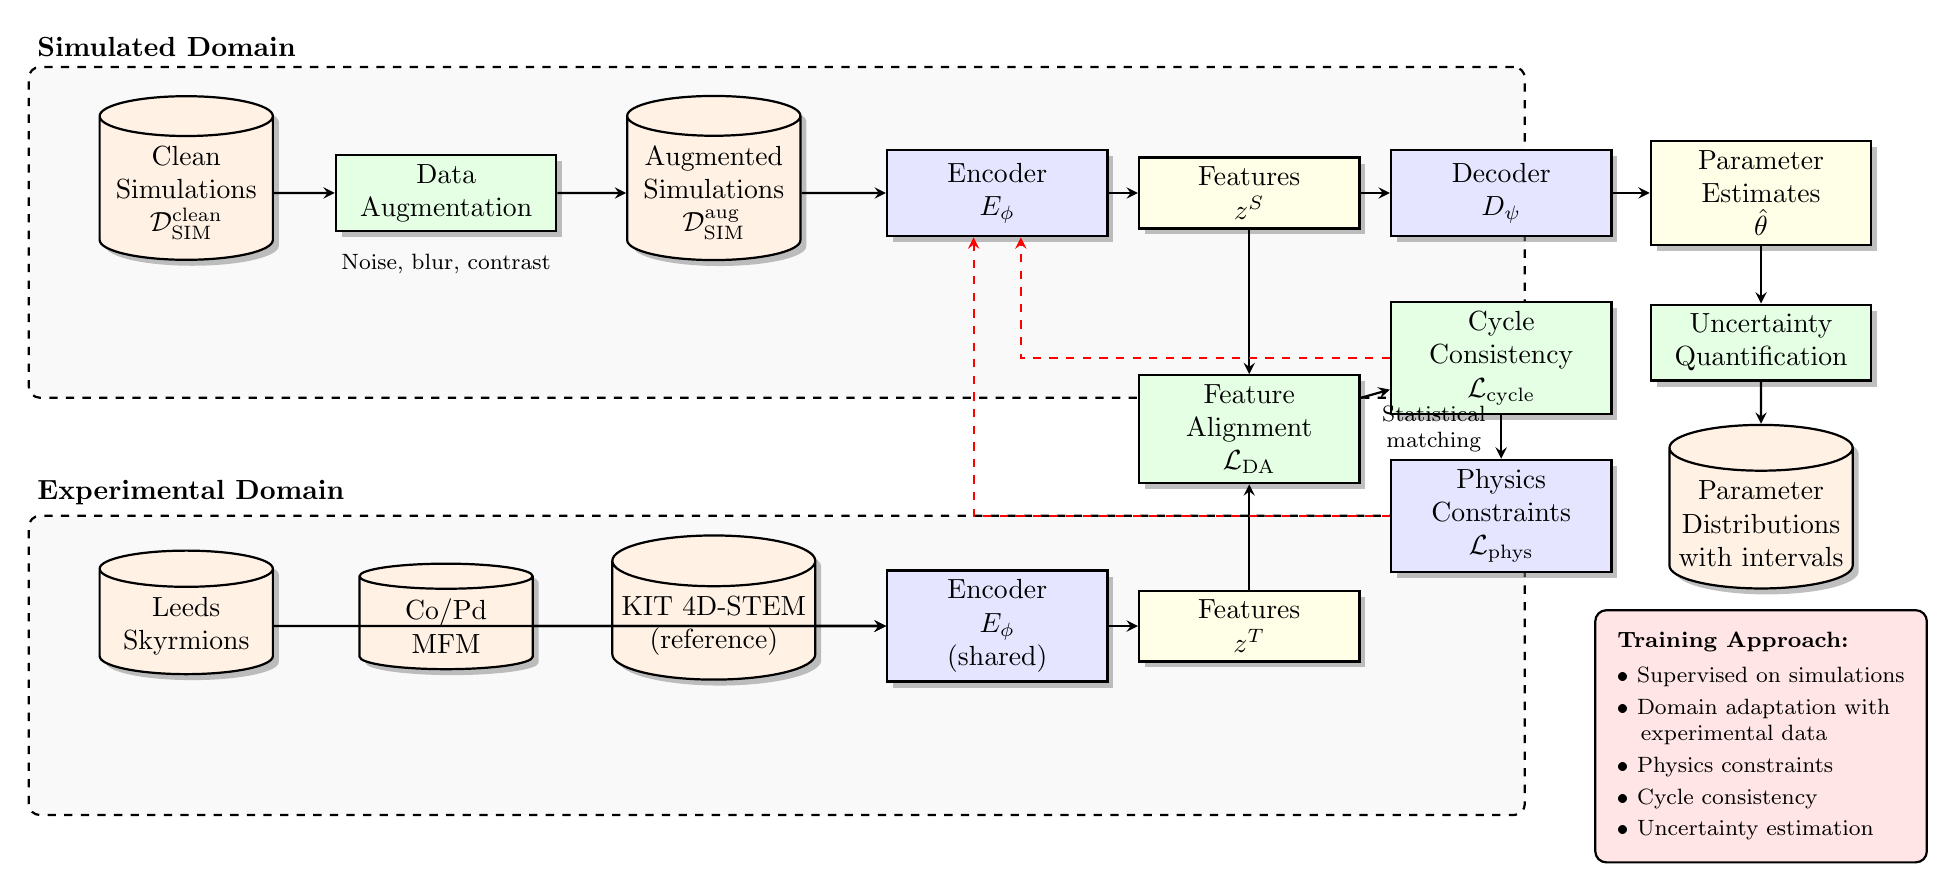
\begin{tikzpicture}[
    node distance=1.8cm and 2.2cm,
    box/.style={rectangle, draw, thick, fill=blue!10, minimum width=2.8cm, minimum height=1.1cm, align=center, drop shadow},
    process/.style={rectangle, draw, thick, fill=green!10, minimum width=2.8cm, minimum height=0.9cm, align=center, drop shadow},
    data/.style={cylinder, draw, thick, fill=orange!10, minimum width=2.2cm, minimum height=1.1cm, align=center, drop shadow, shape border rotate=90, aspect=0.25},
    arrow/.style={->, >=stealth, thick},
    label/.style={font=\small, align=center},
    highlight/.style={rectangle, draw, thick, fill=yellow!10, minimum width=2.8cm, minimum height=0.9cm, align=center, drop shadow},
    domainbox/.style={rectangle, draw, dashed, thick, fill=gray!5, rounded corners, inner sep=10pt},
    infobox/.style={rectangle, draw, thick, fill=red!10, rounded corners, align=left, minimum width=3.5cm, minimum height=2.5cm, inner sep=8pt}
]

% Domain boxes
\node[domainbox, minimum width=19cm, minimum height=4.2cm] (sim_domain) at (0,3.2) {};
\node[above right] at (sim_domain.north west) {\textbf{Simulated Domain}};

\node[domainbox, minimum width=19cm, minimum height=3.8cm] (exp_domain) at (0,-2.3) {};
\node[above right] at (exp_domain.north west) {\textbf{Experimental Domain}};

% Simulated data flow (top)
\node[data] (sim_clean) at (-7.5,3.7) {Clean\\Simulations\\$\mathcal{D}_{\text{SIM}}^{\text{clean}}$};

\node[process] (domain_rand) at (-4.2,3.7) {Data\\Augmentation};

\node[data] (sim_aug) at (-0.8,3.7) {Augmented\\Simulations\\$\mathcal{D}_{\text{SIM}}^{\text{aug}}$};

\node[box] (encoder_sim) at (2.8,3.7) {Encoder\\$E_\phi$};

\node[highlight] (features_sim) at (6,3.7) {Features\\$z^S$};

% Experimental data flow (bottom)
\node[data] (leeds) at (-7.5,-1.8) {Leeds\\Skyrmions};

\node[data] (copd) at (-4.2,-1.8) {Co/Pd\\MFM};

\node[data] (kit) at (-0.8,-1.8) {KIT 4D-STEM\\(reference)};

\node[box] (encoder_exp) at (2.8,-1.8) {Encoder\\$E_\phi$\\(shared)};

\node[highlight] (features_exp) at (6,-1.8) {Features\\$z^T$};

% Feature alignment in the middle
\node[process] (alignment) at (6,0.7) {Feature\\Alignment\\$\mathcal{L}_{\text{DA}}$};

% Decoder and cycle consistency
\node[box] (decoder) at (9.2,3.7) {Decoder\\$D_\psi$};

\node[process] (cycle) at (9.2,1.6) {Cycle\\Consistency\\$\mathcal{L}_{\text{cycle}}$};

\node[box] (physics) at (9.2,-0.4) {Physics\\Constraints\\$\mathcal{L}_{\text{phys}}$};

% Output
\node[highlight] (output) at (12.5,3.7) {Parameter\\Estimates\\$\hat{\theta}$};

\node[process] (prob_inference) at (12.5,1.8) {Uncertainty\\Quantification};

\node[data] (final_output) at (12.5,-0.5) {Parameter\\Distributions\\with intervals};

% Arrows - Simulated flow
\draw[arrow] (sim_clean) -- (domain_rand);
\draw[arrow] (domain_rand) -- (sim_aug);
\draw[arrow] (sim_aug) -- (encoder_sim);
\draw[arrow] (encoder_sim) -- (features_sim);

% Arrows - Experimental flow
\draw[arrow] (leeds) -- (encoder_exp);
\draw[arrow] (copd) -- (encoder_exp);
\draw[arrow] (kit) -- (encoder_exp);
\draw[arrow] (encoder_exp) -- (features_exp);

% Arrows - Feature alignment
\draw[arrow] (features_sim) -- (alignment);
\draw[arrow] (features_exp) -- (alignment);

% Arrows - Decoder and constraints
\draw[arrow] (features_sim) -- (decoder);
\draw[arrow] (decoder) -- (output);
\draw[arrow] (alignment) -- (cycle);
\draw[arrow] (cycle) -- (physics);
\draw[arrow] (output) -- (prob_inference);
\draw[arrow] (prob_inference) -- (final_output);

% Feedback arrows
\draw[arrow, dashed, red] (physics) -| ($(encoder_sim.south) + (-0.3,0)$);
\draw[arrow, dashed, red] (cycle) -| ($(encoder_sim.south) + (0.3,0)$);

% Annotations
\node[label, below=0.15cm of domain_rand, font=\footnotesize] {Noise, blur, contrast};
\node[label, right=0.15cm of alignment, font=\footnotesize] {Statistical\\matching};

% Information box
\node[infobox, font=\footnotesize] at (12.5,-3.2) {
    \textbf{Training Approach:}\\[3pt]
    \textbullet\ Supervised on simulations\\[2pt]
    \textbullet\ Domain adaptation with\\
    \quad experimental data\\[2pt]
    \textbullet\ Physics constraints\\[2pt]
    \textbullet\ Cycle consistency\\[2pt]
    \textbullet\ Uncertainty estimation
};

\end{tikzpicture}
\end{document}
